%
% main.tex -- Paper zum Thema gis
%
% (c) 2019 Hochschule Rapperswil
%
\chapter{Signalanalyse von UHF Teilentladungssignalen im Zeitbereich \label{chapter:gis}}
\lhead{Signalanalyse von UHF Teilentladungssignale im Zeitbereich}
\begin{refsection}
\chapterauthor{Kris Wyss}

\section{Gasisolierte Schaltanlagen}
\rhead{Vorwort}

Gasisolierte Schaltanlagen (GIS) dienen der elektrischen Energieverteilung, dem Schutz der Komponenten und ermöglichen eine sichere Wartung des Energieübertragungsnetzes.
Als Isoliergas wird Schwefelhexafluorid (SF\textsubscript{6}) eingesetzt. SF\textsubscript{6} hat bei Atmosphärendruck eine etwa drei mal so grosse dielektrische Festigkeit (Spannungs-Isolationsvermögen) wie Luft. 
Es besitzt auch um den Faktor 3 bis 4 mal bessere Lichtbogenlöscheingeschaft als Luft. 
Diese Eigenschaften führen zu einer erheblichen Platzeinsparung gegenüber einer luftisolierten Schaltanlage (AIS) \cite{buch:ABB}.
Deshalb und aufgrund anderer Gründen, aufgezeigt in \cite{buch:GIS/AIS}, hat sich der Einsatz von GIS überall dort durchgesetzt wo Boden teuer ist wie zum Beispiel in urbanen Gebieten. 
Bei Leistungsschaltern hat SF\textsubscript{6} nicht ausschliesslich die Aufgabe eines Isoliermediums sondern dient auch als Löschgas des Lichtbogens.
Dieser trägt bis zu mehrere tausend Ampere, wenn grosse Verbraucher vom Übertragungsnetz getrennt werden \cite{buch:ABB}. 

Bei der Quantifizierung der Qualität einer GIS spielt der Begriff Teilentladung (TE) eine wichtige Rolle. 
Wenn das elektrische Feld örtlich über die dielektrische Festigkeit steigt, entstehen Entladungen, welche nur einen Teil der Isolationsstrecke überbrücken und nicht zu einem kompletten Durchschlag führen, daher die Namensgebung Teilentladung \cite{buch:Kuchler}.
Teilentladung im Isolierstoff lässt das Isoliermedium  schneller altern. Dies kann zum dielektrischen Durchschlag führen welcher einen Totalausfall der Anlage zur Folge hat.
Aufgrund dessen ist TE ein wichtiges Qualitätsmerkmal bei Hochspannungskomponenten. 

Tritt Teilentladung auf, werden verschiedene  physikalische Prozesse initiiert. 
Die Entladung hat einen Strompuls zur Folge.
Wegen dem Lichtbogen wird eine ultrahochfrequente (UHF) elektromagnetische Welle emittiert.
Die schnellste gemessene Anstiegszeit des Strompulses in SF\textsubscript{6} liegt bei 24ps.
Dies entspricht einem Frequenzband hoch bis zu 14 GHz \cite{skript:Judd24ps}. 
Aufgrund der schnellen Erhitzung des Gases rund um den Lichtbogen wird eine Schallwelle abgestrahlt. 
Ebenfalls durch die grosse Erhitzung wird das Isoliergas SF\textsubscript{6} zersetzt. 
Somit kann TE chemisch, akustisch oder elektromagnetisch gemessen und lokalisiert werden \cite{skript:StatusReviewPDMeasurement}.
In dieser Arbeit wird auf die Analyse der UHF TE-Signale eingegangen.
Es wird versucht, mittels dem Signalanalyseverfahren kontinuierliche Wavelettransformation (CWT), fehlerspezifische Charakteristiken im Zeitsignal der elektromagnetischen Welle auszumachen.

\section{Fehlerarten und Analyse in GIS}
\rhead{Abschnitt}

TE wird in zwei Grundkategorien unterteilt \cite{buch:Kuchler}, die Innere- und Äussere-TE. 
Die Erstere ist dadurch charakterisiert, dass sich die TE-Quelle im Innern eines festen oder flüssigen Isolierstoffes befindet. 
Bei GIS gehören zur Kategorie der Inneren-TE folgende Fehlerarten, Hohlräume, Risse und Spalten in Isolierstoffe und Delamination zwischen Isolierschichten.
 
Entladungen an äusseren Leiterstrukturen werden als Äussere-TE oder Korona bezeichnet. 
In GIS kommen die zwei Fehler Oberflächenentladung und Koronaentladung aus dieser Kategorie vor.
Oberflächenentladungen treten bei nicht Einhalten der Herstellungstoleranzen zwischen leitendem und isolierendem Material auf.
Eine weitere Quelle sind potenzialfrei leitende Partikel auf festen Isolierstoffen.
Spitzen und scharfe Kanten an spannungsführenden- und leitfähigen-Teilen auf Erdpotenzial führen zu Koronaentladung \cite{buch:Kuchler, skript:AeussreTE, skript:InnereTE}.
Weiterführende Literatur zu diesem Thema
\begin{itemize}
	\item \citeauthor{buch:Kuchler} \cite{buch:Kuchler}
	\item \citeauthor{skript:AeussreTE} \cite{skript:AeussreTE}
	\item \citeauthor{skript:InnereTE} \cite{skript:InnereTE}  
\end{itemize}
kann in den Referenzen gefunden werden.
In dieser Arbeit werden UHF TE-Signale von Oberflächenentladung und Hohlraumentladungen analysiert. 
In dem folgenden Abschnitten werden die physikalischen Hintergründe von zwei Entladungsarte aufgezeigt und die herkömmliche Fehleranalyse beschrieben. 

\subsection{Oberflächenentladung}

Diese Entladungsart entsteht, wenn an Oberflächen von festisolierstoffen hohe elektrische Feldstärken auftreten. 
Dies kann konstruktionsbedingt oder Aufgrund fehlerhaften Montage entstehen.
Befindet sich ein Spitze oder scharfe Kante oberhalb eines Festisolierstoffes oder ein loser metallischer Partikel auf einem Isolierstoff, dann entladen sich die Stromimpulse über das Isoliermaterial. 
In Abbildung \ref{fig:oberflaechenentladung} ist ersichtlich, dass die Art der TE einer Koronaentladung entspricht. 
Jedoch verteilen sich die Elektronen nicht im Gasraum sondern sie gleiten über die Isolierfläche welche als helle Fläche in der Abbildung erkennbar ist.
\begin{figure}
    \centering
	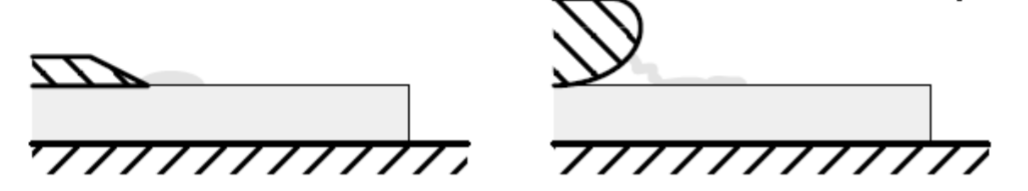
\includegraphics[width=0.7\linewidth]{papers/gis/Bilder/Oberflaechenentladung}
	\caption{Zwei Anordnungen von Oberflächenentladungen \cite{buch:Kuchler}}
	\label{fig:oberflaechenentladung}
\end{figure}
Das Ersatzschaltbild (ESB) \ref{fig:M1} besteht aus einer Kapazität $C$ parallel zu einer Funkenstrecke $F$ und einem Widerstand $R$ in Serie. 
Der Pfeil symbolisiert die Spitze an welcher ein inhomogenes elektrisches Feld ansteht.
	Wenn das Feld über der Kapazität einen kritischen Wert erreicht entlädt sich die gespeicherte Energie in der Funkenstrecke gegen Erde.
Dieser Prozess kann sich bei Wechselspannung mehrmals pro Halbwelle wiederholen \cite{skript:AeussreTE}. 
\begin{figure}
\centering
\begin{circuitikz} [scale=0.6] \draw

(0,1)node[vee]{Spitze} (0,1)--(0,0)
to[C=$C$, v=$u_c(t)$] (0,-3)
to[R=$R$]  (0,-5)
node[rground]{}
(0, 0) -- (3, 0.0) -- (3, -1) 
to[american gas filled surge arrester=$F$] (3, -2) -- (3, -3) -- (0,-3)
			(-2, 0) to[open, v=$u(t)$] (-2, -4)
	;
\end{circuitikz}
\caption{Ersatzschaltbild Koronaentladung} \label{fig:M1}
\end{figure}


\subsection{Hohlraumentladung}

Hohlraumentladungen in GIS kommen am häufigsten aufgrund von Hohlräumen im Isolierstoff vor. 
Hohlräume entstehen beim Herstellungsprozess der Isolatoren. Während dem Abkühlprozess kann es zu Diffusionsvorgängen in der
Isoliermasse kommen.
Dadurch können sich gasgefüllte Hohlräume im Isolierstoff ausbilden. 
Oft wird im Model von runden, luftgefüllten Hohlräumen mit niedriger elektrischer Festigkeit ausgegangen. 
Jedoch sind in der Praxis die genauen geometrischen und dielektrischen Eigenschaften nicht bekannt, da die Fehlstelle nicht zugänglich ist. 
In Abbildung \ref{fig:hohlraum} sind diverse Hohlräume 1--3 illustriert. Unter der Nummer 1 sind klassische runde oder ellipsenförmige Lunker ohne Elektrodenkontakt abgebildet. 
Die beiden anderen Hohlräume haben Elektrodenkontakt und die Nummer 3 stellt eine Ablösung von der leitfähigen Elektrodenschicht dar  \cite{buch:Kuchler, skript:InnereTE}.

Elektrisch wird die Fehlerart mit dem Ersatzschaltbild gemäss \ref{fig:M2} modelliert. 
Die Kapazität $C\textsubscript{0}$ stellt dabei die Gesamtkapazität über der Isolierstrecke dar und $C\textsubscript{h}$ ist die Hohlraumkapazität, welche die Fehlerstelle abbildet.
Die Spannung $u\textsubscript{h}(t)$ folgt der äusseren Spannung $u(t)$ bis die Zündspannung erreicht ist. 
Bei dieser Spannung hat die Feldstärke über der Hohlraumkapazität einen kritischen Wert überschritten und die Energie, bei vorhanden sein eines Startelektrons, entlädt sich über die Funkenstrecke $F$.
Die Spannung über $u\textsubscript{h}(t)$ sinkt bis zur Löschspannung, danach kann sich der selbe Vorgang mehrere Male pro Halbwelle wiederholen. 
Über die Serienkapazität $C\textsubscript{s}$ wird die Hohlraumkapazität $C\textsubscript{h}$ via einem kapazitiven Verbschiebestrom nachgeladen \cite{buch:Kuchler}. 

\begin{figure}
	\centering
	\begin{circuitikz} [european, scale=0.5] 
		\draw
		(-3,0)node[vcc]{Hochspannung} (-3,0)--(-3,-1)
		to[C=$C\textsubscript{0}$] (-3,-3) -- (-3,-4)
		node[rground] {}
		(-3.5, 0) to[open, v=$u(t)$] (-3.5, -4)
		
		(0,0)
		to[C=$C\textsubscript{s}$] (0,-2) 
		to[C=$C\textsubscript{h}$, v=$u\textsubscript{h}(t)$] (0,-4)
		node[rground]{}
		
		(-3,0) --(0, 0)
		
		(0, -2) -- (3,-2) to[american gas filled surge arrester=$F$] (3, -4)
		node[rground]{} 
		;
	\end{circuitikz}
	\caption{Ersatzschaltbild Hohlraumentladung} 
	\label{fig:M2}
	\end{figure}

\begin{figure}
	\centering
	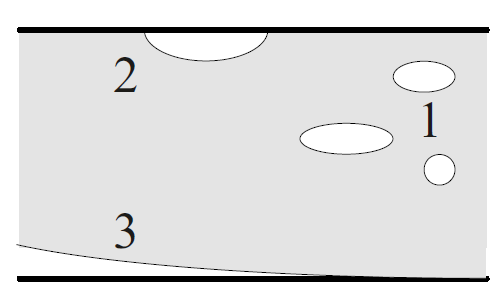
\includegraphics[width=0.5\linewidth]{papers/gis/Bilder/Hohlraum}
	\caption[]{Bsp. von geometrisch verschedenen Hohlräume mit und ohne Elektrodenkontakt \cite{buch:Kuchler}}
	\label{fig:hohlraum}
\end{figure}
  
\subsection{Herkömmliche Fehleranalyse}

Um die fehlerspezifischen physikalisch und elektrotechnischen Phänomene bildlich darzustellen, muss ein Bezug hergestellt werden zwischen dem Entladungszeitpunkt und dem Phasenwinkel der Hochspannung, welche am Prüfling anliegt. 
Mit diesen Daten wird ein phasenaufgelöstes Teilentladungsmuster (PRPD: Phase-resolved partial discharge) erstellt. 
In dem Bild wird die Korrelation zwischen der Phasenlage $\phi$, Amplitudenhöhe $Q$ und der Anzahl Entladungen $N$ dargestellt \cite{buch:UHFSignale}. 
In Abbildung \ref{fig:PRPDAlg} sind diese Zusammenhänge aufgezeigt und in Abbildung \ref{fig:PRPDHohl} 
ist ein Beispiel dargestellt wie das Muster einer typischen Oberflächenentladung aussieht. 
Im oberen Bereich ist die Phasenlage der angelegten Spannung aufgezeigt und im unteren Bildteil sind die Entladungen gemäss dem in Abbildung \ref{fig:PRPDAlg} gezeigten Algorithmus ersichtlich.
Die Muster werden über den Zeitraum von einer bis mehreren Minuten aufgezeichnet.
\begin{figure}
	\centering
	\begin{minipage}{.5\textwidth}
		\centering
		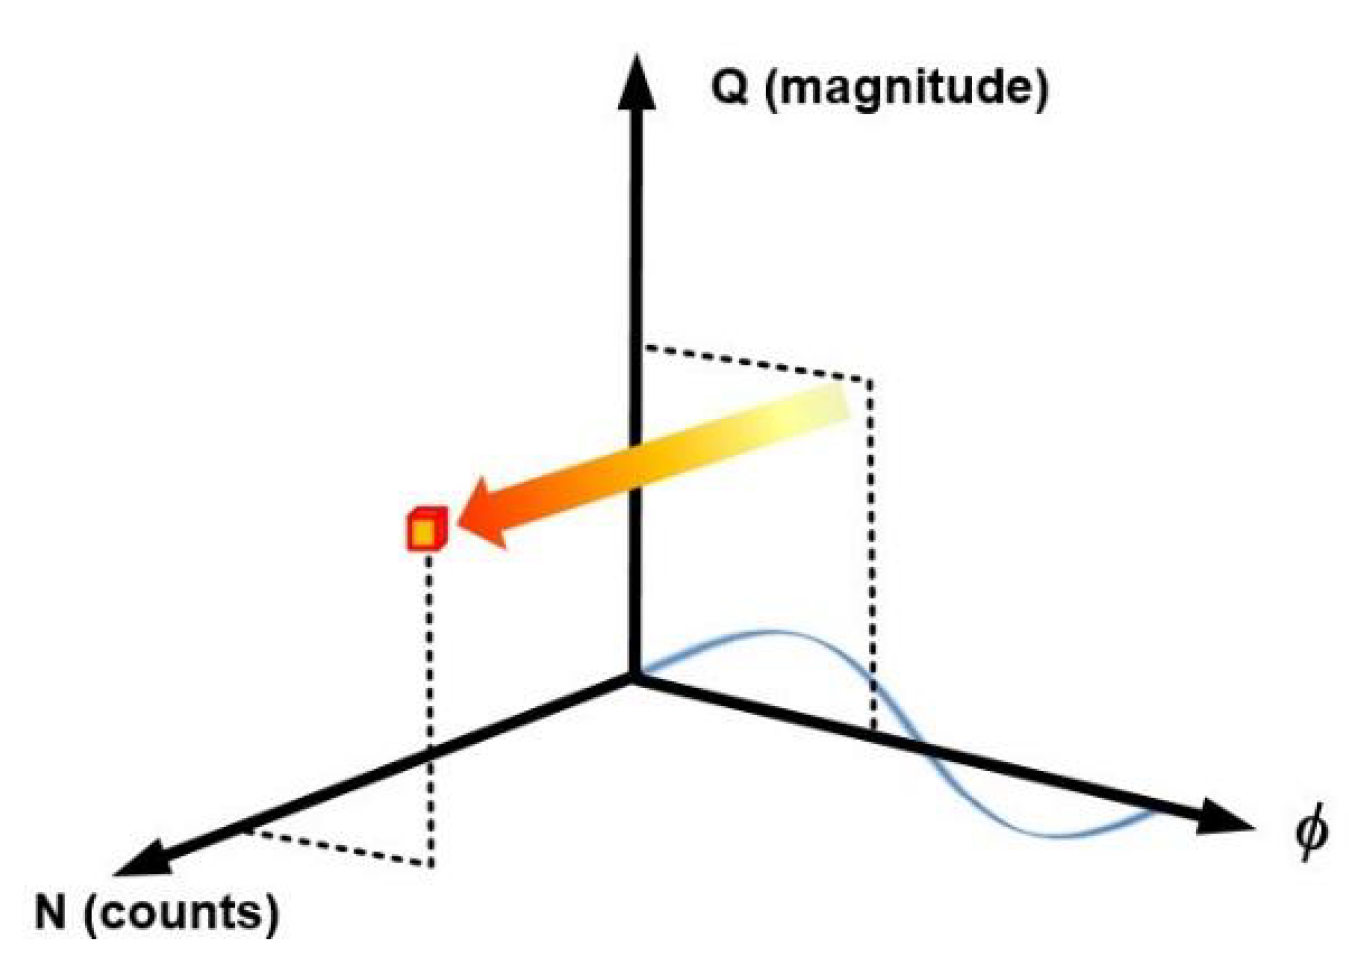
\includegraphics[width=.9\linewidth]{papers/gis/Bilder/PERP}
		\captionof{figure}{PRPD Algorithmus \cite{report:ABBOnSite}}
		\label{fig:PRPDAlg}
	\end{minipage}%
	\begin{minipage}{.5\textwidth}
		\centering
		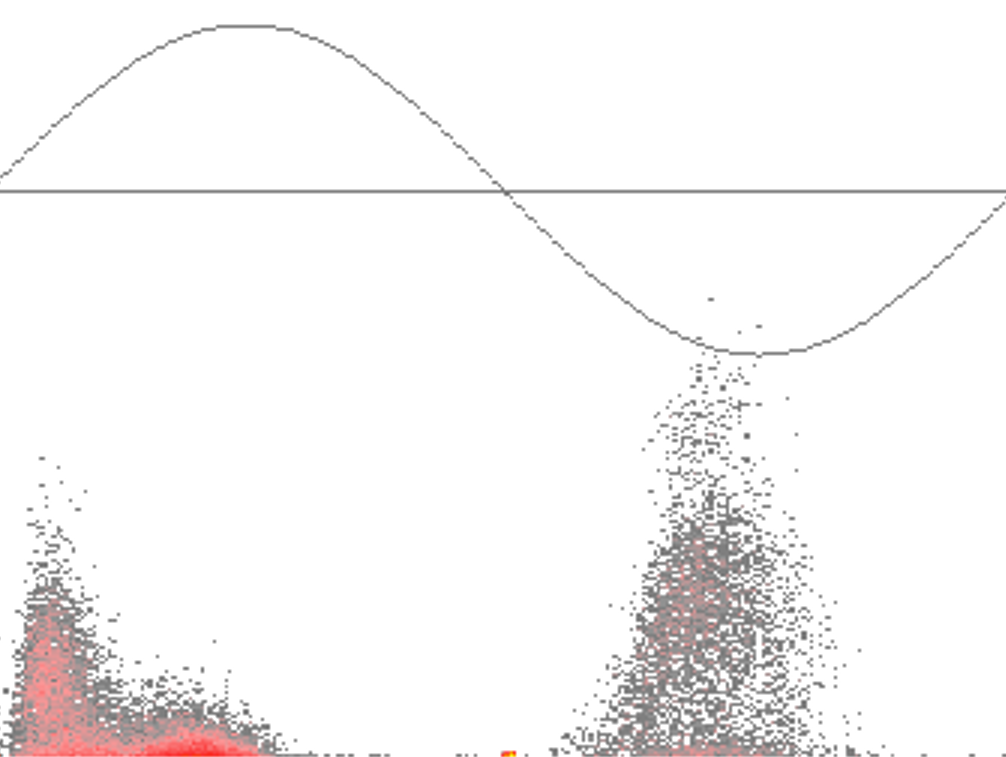
\includegraphics[width=.8\linewidth]{papers/gis/Bilder/OberflaechenentladungPRPD}
		\captionof{figure}{Typisches PRPD-Muster}
		\label{fig:PRPDHohl}
	\end{minipage}
\end{figure}


\section{Messkette}
\rhead{Abschnitt}
In dieser Arbeit wird untersucht, ob mit der kontinuierlichen Wavelet Transformation fehlerspezifische Merkmale im Zeitsignal auszumachen sind. 
Dafür ist es wichtig, dass der Messpfad von der Fehlerursache bis zum Oszilloskop bekannt ist. 
Die untersuchten Signale wurden bei einer Vor-Ort Abklärung, an einer Anlage die im Betrieb war, aufgezeichnet.  
Im ersten Abschnitt wird auf den Signalpfad innerhalb der GIS eingegangen und in einem zweiten auf die Messkette ausserhalb.
\subsection{Messkette innerhalb GIS}
Bei der Fehlstelle am Punkt 0 in Abbildung \ref{fig:messketteingis} wird aufgrund der schnellen Entladung des Strompulses eine elektromagnetische Welle abgestrahlt. 
Das Signal besitzt Frequenzanteile bis in den zweistelligen GHz Bereich. 
In erster Näherung wird die GIS oft als Koaxialkabel modelliert. 
Diese Vereinfachung ist jedoch nicht ausreichend, da Reflexionsphänomene auftreten. 
An diverser Unstetigkeitsstellen in einer GIS, wie Epoxidisolatoren Punkt 1, Verzweigungen Punkt 2,  Änderung der Leiterdurchmesser Punkt 3, schaltenden Elementen und den Enden der Anordnung, ändert der Wellenwiderstand und es kommt zu Reflexionen der Welle.
Eine weitere Signalverzerrung entsteht auf Grund von Dispersionsphänomenen, die sich besonders in bei den Epoxidisolatoren am Punkt 1 bemerkbar machen. 
Aufgrund von all den oben erwähnten Effekten erfährt die Signalleistung auf dem Signalpfad eine hohe Dämpfung.
In Abbildung \ref{fig:messketteingis} sind einige approximative Dämpfungswerte für GIS Komponenten angezeigt  \cite{report:PDBasicABB}.
Eine GIS hat an diversen Stellen breitbandige Koppelantennen wei bei Punkt 4, damit die UHF Teilentladungssignale für Fehleranalysen ausgekoppelt werden können \cite{buch:UHFSignale, skript:Judd24ps, buch:Kuchler}.
\begin{figure}
	\centering
	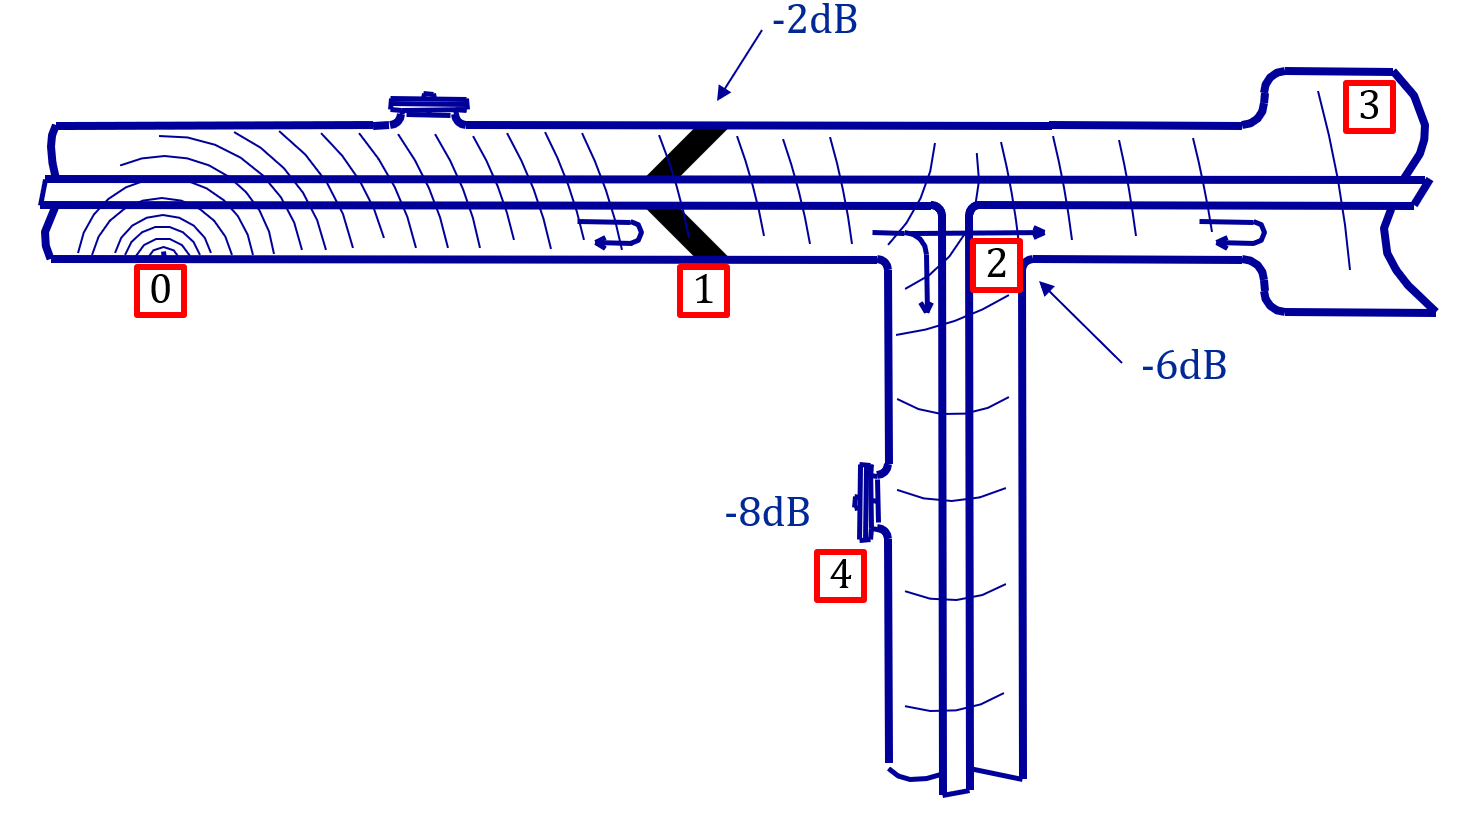
\includegraphics[width=0.5\linewidth]{papers/gis/Bilder/MessketteInGIS}
	\caption{Unstetigkeitsstellen GIS \cite{report:PDBasicABB}}
	\label{fig:messketteingis}
\end{figure}
\subsection{Messkette ausserhalb GIS}
Nach der Koppelantenne ist ein Hochpassfilter mit der Eckfrequenz 83MHz geschaltet.
Dieser dient zum Schutz der dahinterliegenden Messgeräte.
Falls es zu einem dielektrischen Durchschlag kommt, werden die hochenergetischen Signalanteile gegen Erde abgeleitet.
Danach wird das Signal mit 50dB verstärkt.
Die 50$\Omega$ Signalkabel werden an einen Multiplexer angeschlossen. 
Der Multiplexer ermöglicht eine schnelle Auswahl zwischen vielen verschiedenen Koppelantennen damit das erwünschte Signal auf einem Frequenzanalysator oder Oszilloskop angezeigt werden kann. 
Für die untersuchten Daten sind die Zeitsignale mit einem 10GS/s Oszilloskop mit 2GHz Bandbreite aufgezeichnet worden.
Die Abtastzeit wurde für alle Signale gleich gewählt und liegt bei 100ps. 
\begin{figure}
	\centering
	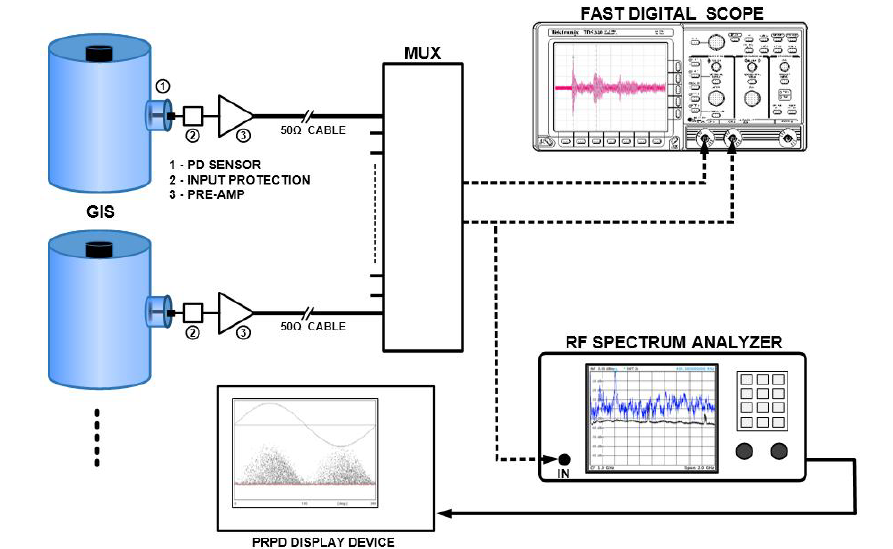
\includegraphics[width=0.9\linewidth]{papers/gis/Bilder/MessketteAusGIS}
	\caption{Messkette \cite{report:ABBOnSite}}
	\label{fig:messketteausgis}
\end{figure}

 
\section{Datenbearbeitung}
\rhead{Abschnitt}

Die analysierten Zeitsignale sind während Laufzeitmessungen (TOF: Time of flight) aufgenommen worden. 
Bei einer TOF Messung sind nur die Anfänge der Signale von Interesse.
Dies bedeutet, dass selten die ganze Einhüllende aufgezeichnet wird und oft werden die Analog Digital Wander (ADC) übersteuert. 
Somit sind die Signale nicht brauchbar für eine CWT.
Es wurden aus ca. 700 Aufzeichnungen vier passende Signale gefunden, welche genug lange aufgezeichnet wurden und bei denen die Signalamplituden nicht abgeschnitten sind. 
Mit Hilfe des Kundenberichtes, welcher die PRPD Muster enthält und den Handnotizen, auf welchen die Zeitstempel und Ortsangaben vermerkt sind, konnten die Zeitsignale den Fehlerquellen zugeordnet werden.
Von den vier Signalen sind je zwei von den Fehlerarten Hohlraumentladung und Oberflächenentladung.
\begin{figure}
	\centering
	
	\begin{subfigure}
		\centering
		\begin{tikzpicture}
		\begin{axis}
		[
		title = a),
		width = 10cm,
		height = 3.5cm,
		xmin = -1.5e-7,
		xmax = 0.8e-6,
		xlabel=time (s),
		ylabel=voltage (V)
		]
		\addplot [red] coordinates{(-1.5e-7, 0.03) (8e-7, 0.03)};
		\addplot [black, samples=10000] file {papers/gis/Messdaten/Data.txt};
		\node[pin=145:{Start}] at (axis cs:0,0) {};
		\node[pin=155:{Treshold}] at (axis cs:6e-7,0.03) {};
		\end{axis}
		\end{tikzpicture}
	\end{subfigure}
	\begin{subfigure}
		\centering
		\begin{tikzpicture}
		
		\begin{axis}
		[
		title = b),
		width = 10cm,
		height = 3.5cm,
		xmin = -0.15e-7,
		xmax = 3e-7,
		xlabel=time (s),
		ylabel=voltage (V)
		]
		\addplot [black, samples=10000] file {papers/gis/Messdaten/Data.txt};
		\end{axis}
		\end{tikzpicture}
	\end{subfigure}	
\caption{a) Vor Harmonisierung b) Nach Harmonisierung}
\label{fig:Zeitsig}
\end{figure}

Damit die Messungen sinnvoll miteinander vergleichbar sind, wurden einige Datenaufbereitungen im Matlabcode implementiert.
Dies dient zur Harmonisierung der zu untersuchenden Signale (siehe Abbildung \ref{fig:Zeitsig}). 
Auf diese wird im Folgenden kurz eingegangen.

\subsection{Thresholding}
Durch Transformieren von vielen Signalen hat sich gezeigt, dass der informative Bereich, wo die CWT relevante Muster hervorbringt, in den ersten 300ns ist.
Bei einer Abtastzeit von 100ps entspricht dies 3000 Datenpunkte welche den Datenvektor $v_d$ bilden.
Um den Startpunkt des Signals zu extrahieren wurde ein Thresholdlevel, in Deutsch Schwellwert, mit folgendem Algorithmus implementiert:

Aus den ersten 300 Datenwerte wird der Vektorindex $v_\text{max}$ mit dem grössten absoluten Wert ermittelt.
Der Thresholdlevel
\begin{equation}
\text{Tresholdlevel} = 3\cdot v_\text{max}^2
\end{equation}
wird durch Quadrieren von Wert in $v_{max}$ und Multiplikation mit 3 festgelegt.
Der Startpunkt wird ermittelt, indem das erste Vektorelement im Datenvektor $v_d$ gesucht wird, welches diesen überschreitet.
Dazu wird der gesamte Datenvektor 
\begin{equation}
\text{$v_d^2$}
\end{equation}
quadriert.
Mit dem Quadrieren wird ein grösserer Signal-Rausch-Abstand (SNR) erzielt und negative Werte werden mit einbezogen.

\subsection{Frequenzinterpretation}
Um die CWT Muster aussagekräftiger darzustellen wird auf der $y$-Achse nicht die Dilatationsskalierungen angezeigt. 
Stattdessen wird ein Rückschluss auf die Frequenz abgeleitet. 
Diese darf jedoch nur als Approximation betrachtet werden.
Aufgrund der Unschärferelation entspricht in einer CWT die Frequenzauflösung nicht der Auflösung einer Fourier-Transformation. 
Die Frequenzapproximation 
\begin{equation}
F_a=\dfrac{F_c}{a}
\end{equation}
ist definiert durch die Division der Mittelfrequenz $F_c$ des entsprechenden Wavelets und dem Wavelet-Dilatationsfaktor $a$.

Diese wird durch den höchsten Wert des Skalarproduktes 
\begin{equation}
F_c(t/a) = \max_a\langle \psi(t),\sin (t/a)\rangle
\end{equation}
zwischen dem Wavelet $\psi$ und dem Sinus berechnet.
Wobei der Sinus mit dem Dilatationsfaktor $a$ gestreckt wird.
Die Variable $a$ steht für den Dilatationsskalierungsfaktor. 
Damit wird erzielt das die $y$-Achse mit der approximierten Frequenz $F_a$ skaliert werden kann.
In Abbildung \ref{fig:Mittenfrequ} ist die Mittenfrequenz von einem Daubechies-Wavelet Nr. 8 (db8) dargestellt.
Die Abtastfrequenz ist 1Hz und die Center Frequency korrespondiert mit dem Wavelet-Dilatationsfaktor 1.   

\begin{figure}
	\centering
	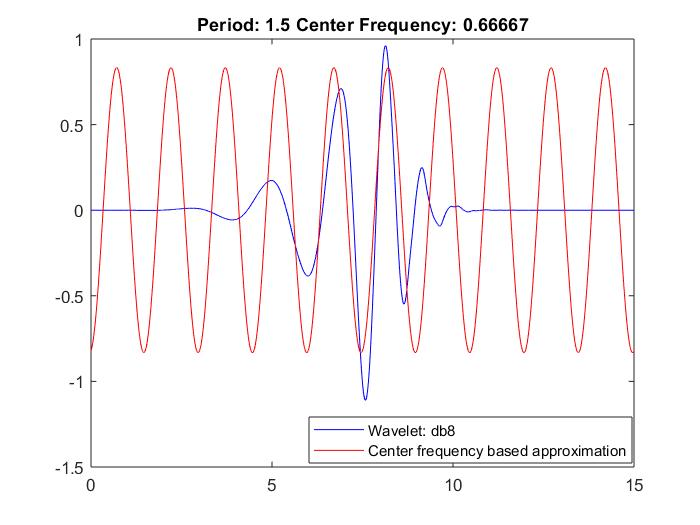
\includegraphics [width=0.7\linewidth] {papers/gis/Bilder/Mittenfrequenz}
	\caption{Mittelfrequenzermittlung db8 für Scale=1}
	\label{fig:Mittenfrequ}
\end{figure}


\section{Auswertung kontinuierliche Wavelettransformation}
\rhead{Abschnitt}
In folgendem Abschnitt wird beschrieben, wie die Auswertung der vier Fehlsignalen von den zwei verschiedenen Fehlerarten angegangen wurde. Auf die Resultate und Erkenntnisse aus diesen wird ebenfalls eingegangen. 
\subsection{Auswertung und Resultat}
Da bei dem zu untersuchenden Problem nicht klar war, nach was genau gesucht werden sollte, wurden Wavelets für verschiedene Signalcharakteristiken verwendet.
\begin{itemize}
	\item Haar
	\item Daubechies 
	\item Symlets
	\item Komplex Gaussian
	\item Real und komplex Morlet
\end{itemize}
Es sind von jeder Familie mit verschiedenen Exponaten jeweils zwei CWT Plots erstellt worden. 
Die zwei dazu verwendeten Zeitsignale gehörten je zu einer der beiden Fehlerarten Oberflächenentladung oder Hohlraumentladung.
Visuell sind die zwei Plots miteinander verglichen worden.
Bei Auffälligkeiten wurden zwei weitere Zeitsignale transformiert, um diese zu bestätigen.
Es konnte jedoch keine typische Bildcharakteristik gefunden werden, welche nur bei einer Fehlerart auftritt.

\subsection{Erkenntnisse Waveleteigenschaften}
Mit der Wahl des Wavelet kann bestimmt werden ob mehr Zeit $\Delta t$ oder Frequenzauflösung $\Delta f$ gewünscht ist. 
Der Grund dafür ist die küpfmüllersche Unbestimmtheitsrelation oder auch Unschärferelation der Nachrichtentechnik genannt
\begin{equation}
\Delta t \cdot \Delta f = k
\qquad\text{mit}\qquad
k = 1
\end{equation}
welche besagt das nicht gleichzeitig beide Auflösungen beliebig genau sein können.
Noch klarer wird der Zusammenhang bei der Grenzfallbetrachtung, wenn auf ein Diracstoss mit unendlich kurzer Zeitdauer die Fouriertransformation angewendet wird.
Es resultiert ein gerades Frequenzspektrum über den kompletten Frequenzbereich.

\begin{figure}
	\centering
	\centering
	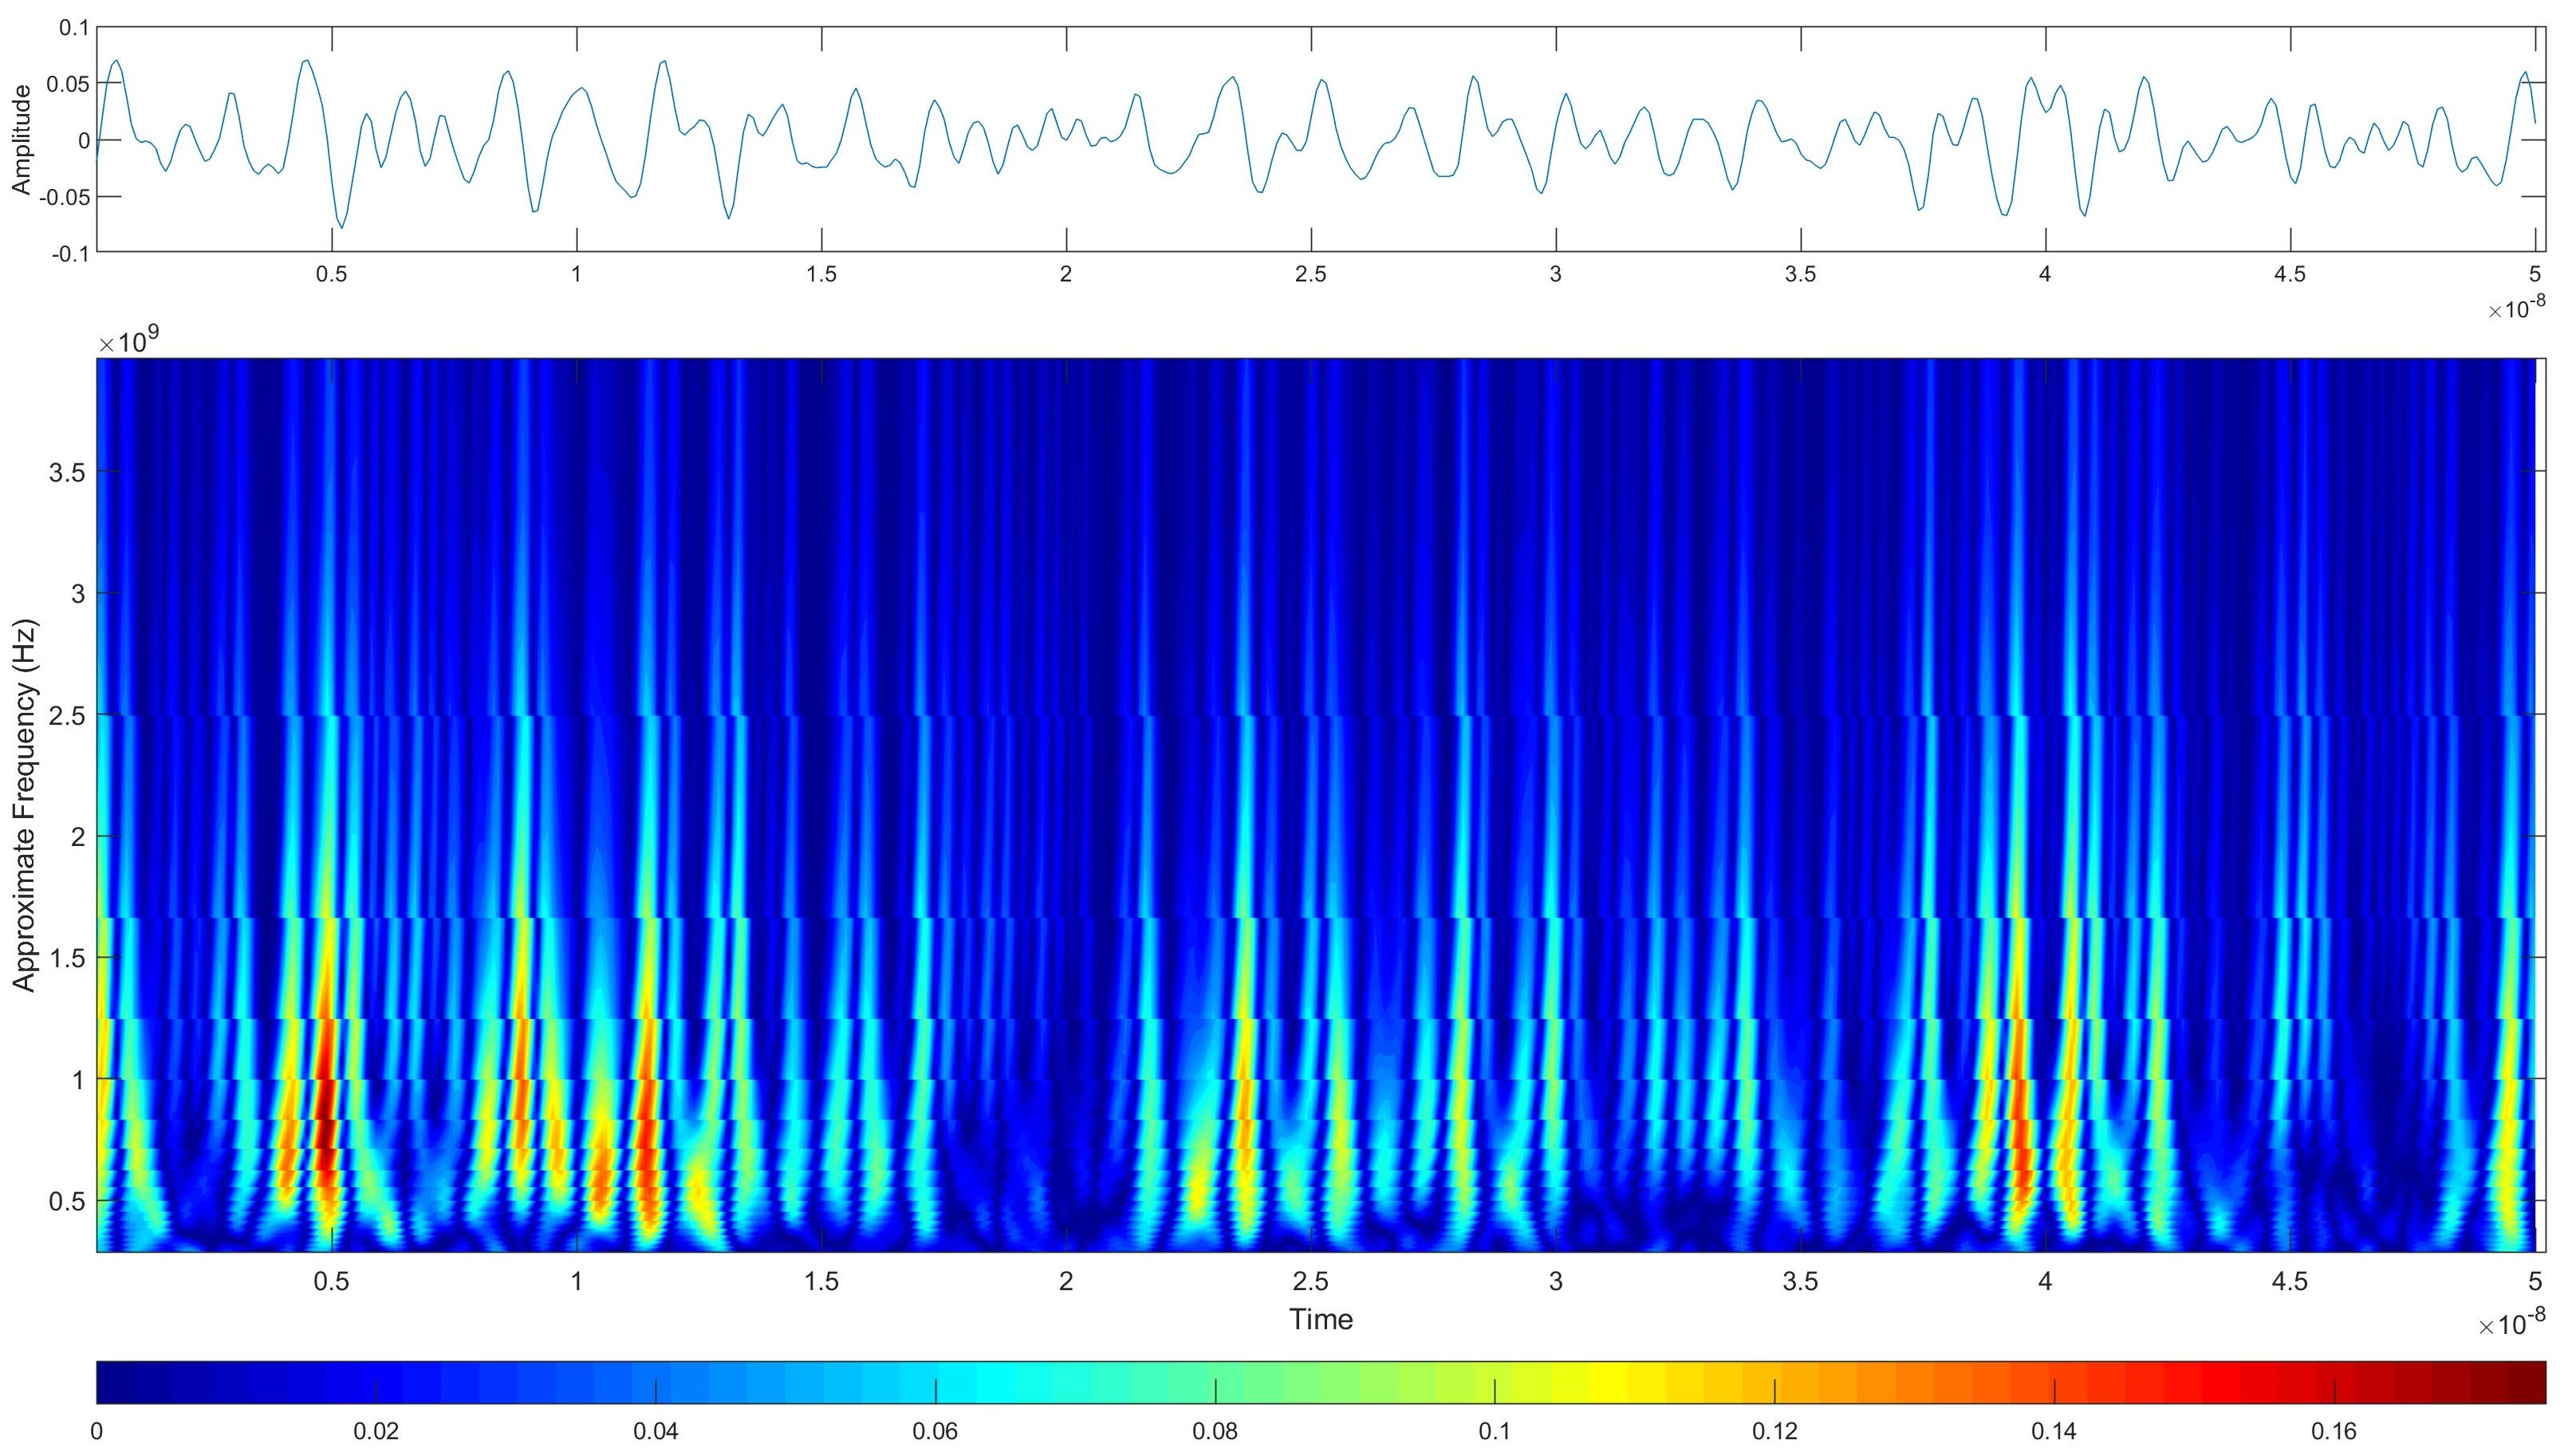
\includegraphics[width=1\linewidth]{papers/gis/Bilder/UnschRelHaar}
	\captionof{figure}{CWT Plot Haar-Wavelet}
	\label{fig:UnschRelHaar}
\end{figure}
\begin{figure}
	\centering
	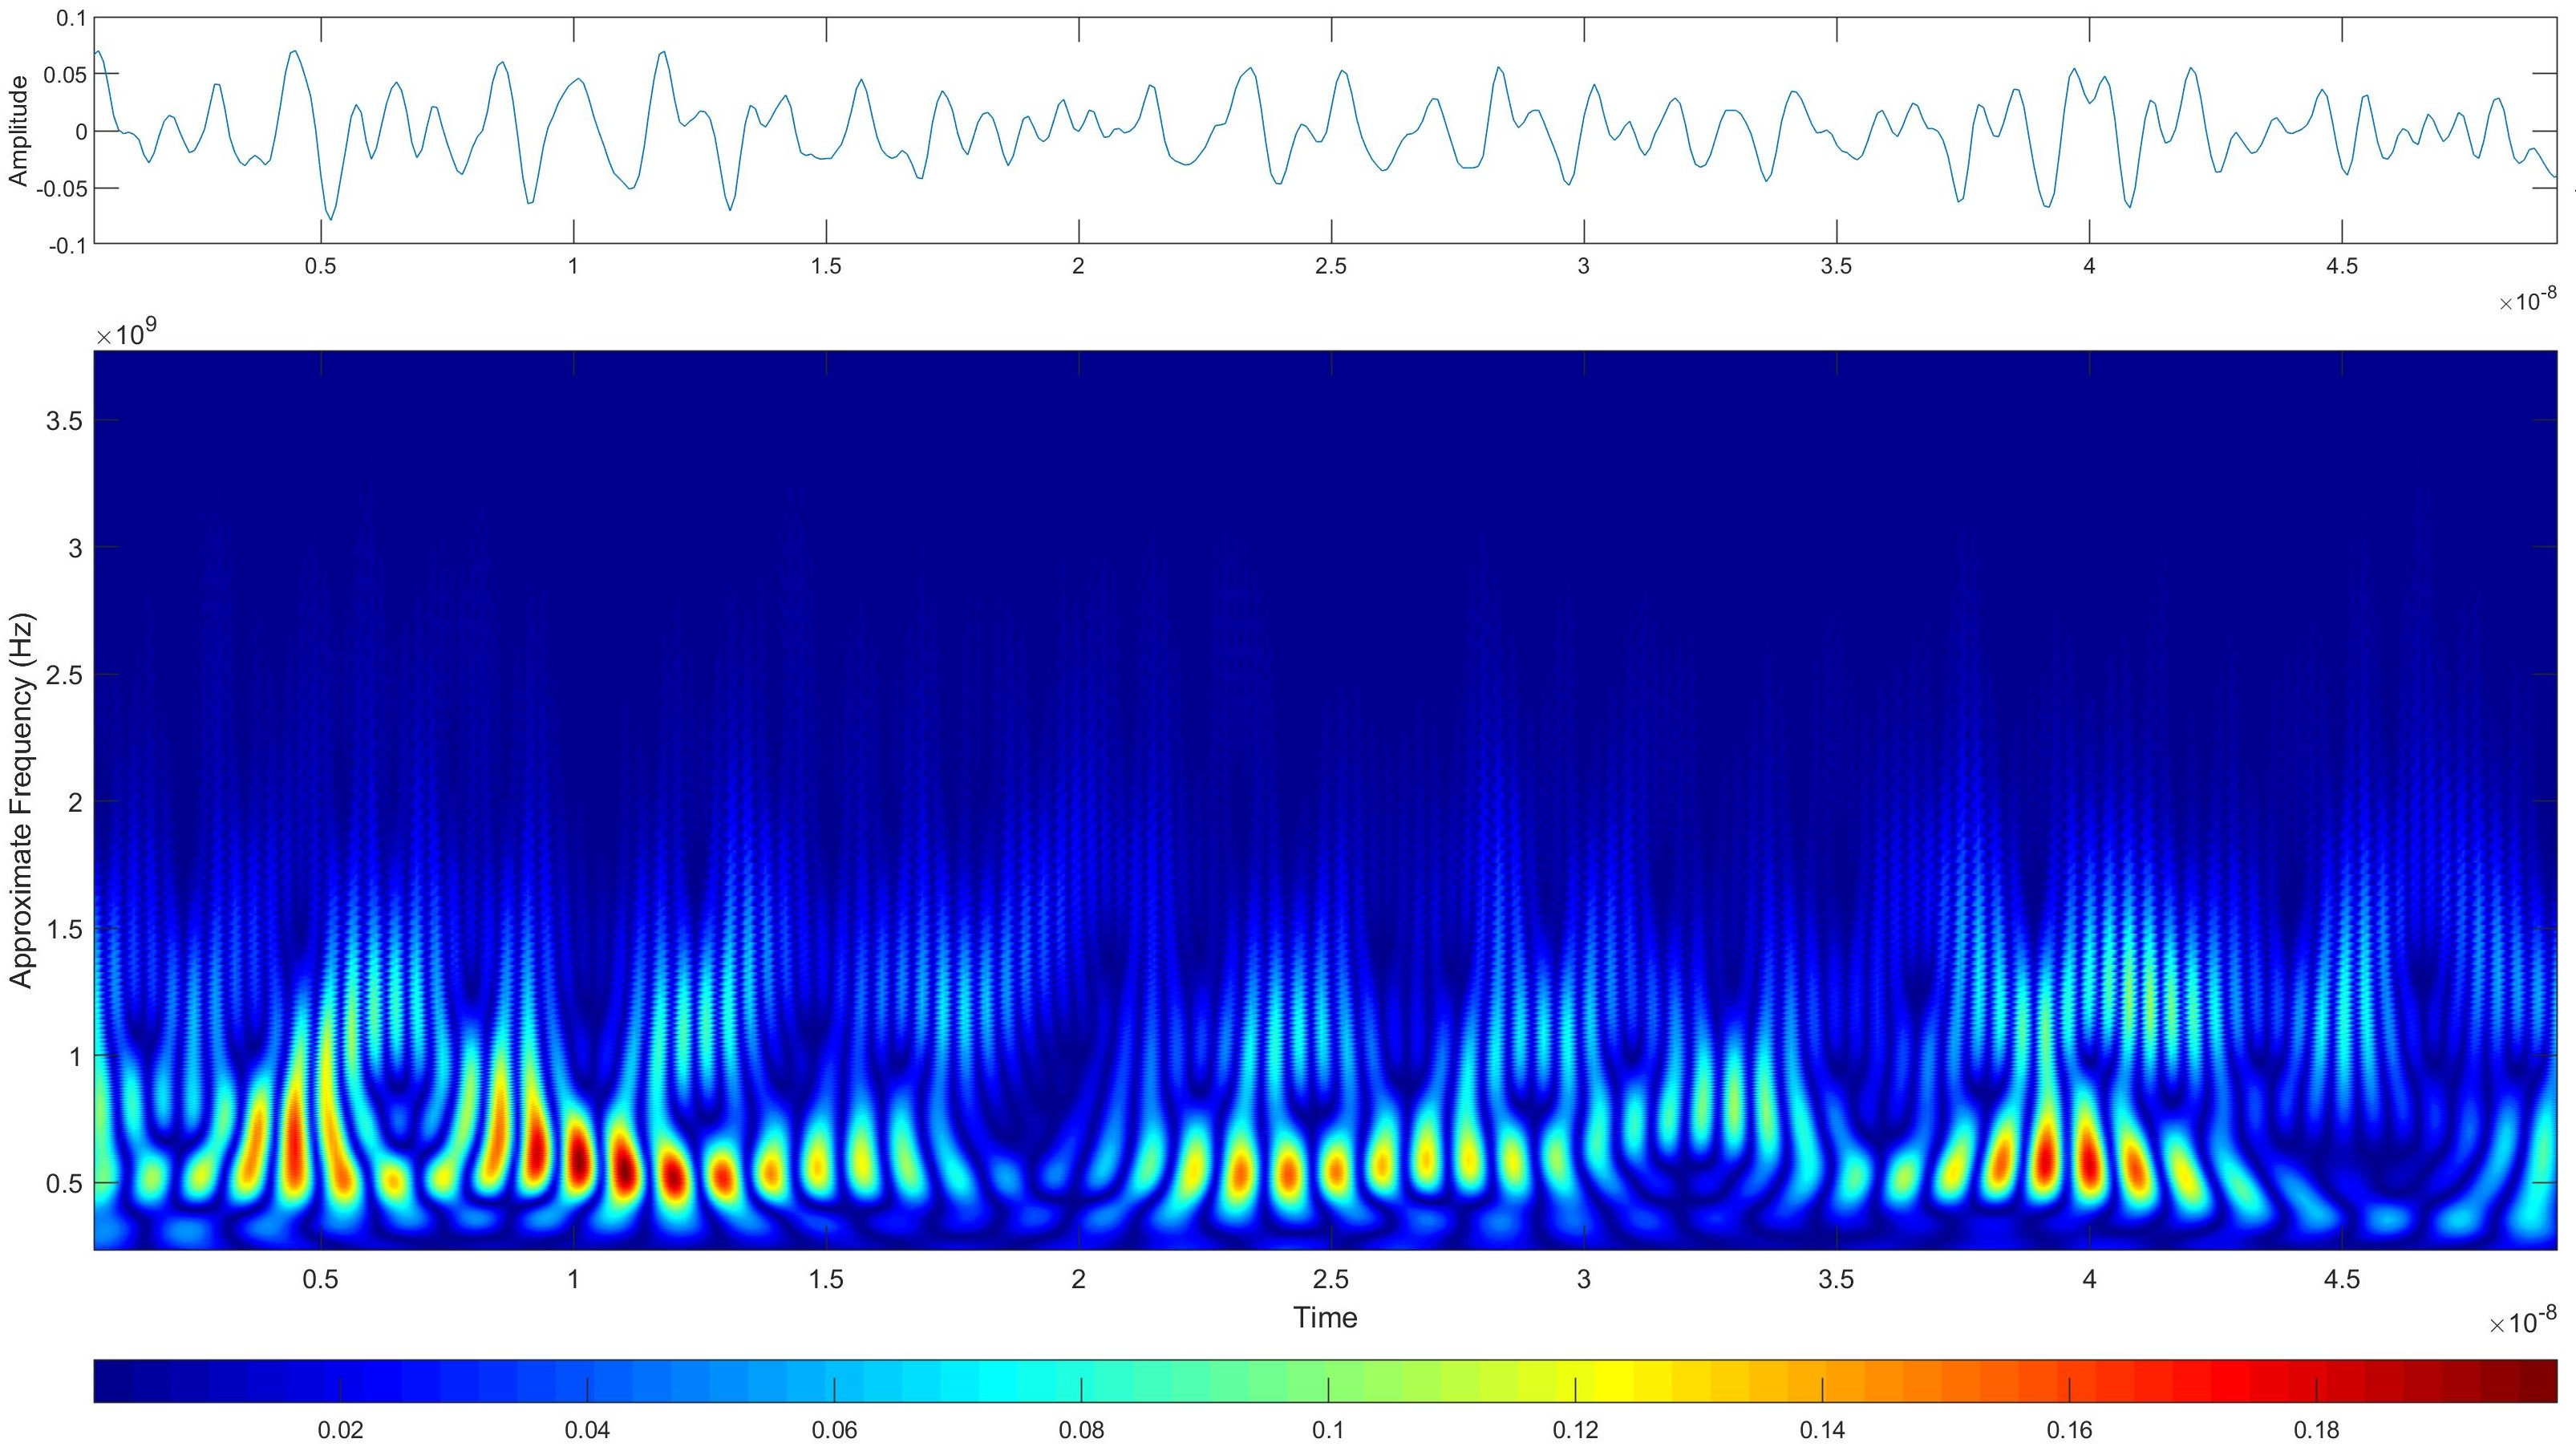
\includegraphics[width=1\linewidth]{papers/gis/Bilder/UnschRelMorl}
	\captionof{figure}{CWT Plot Morlet-Wavelet}
	\label{fig:UnschRelMorl}
\end{figure}
\begin{figure}
	\centering
	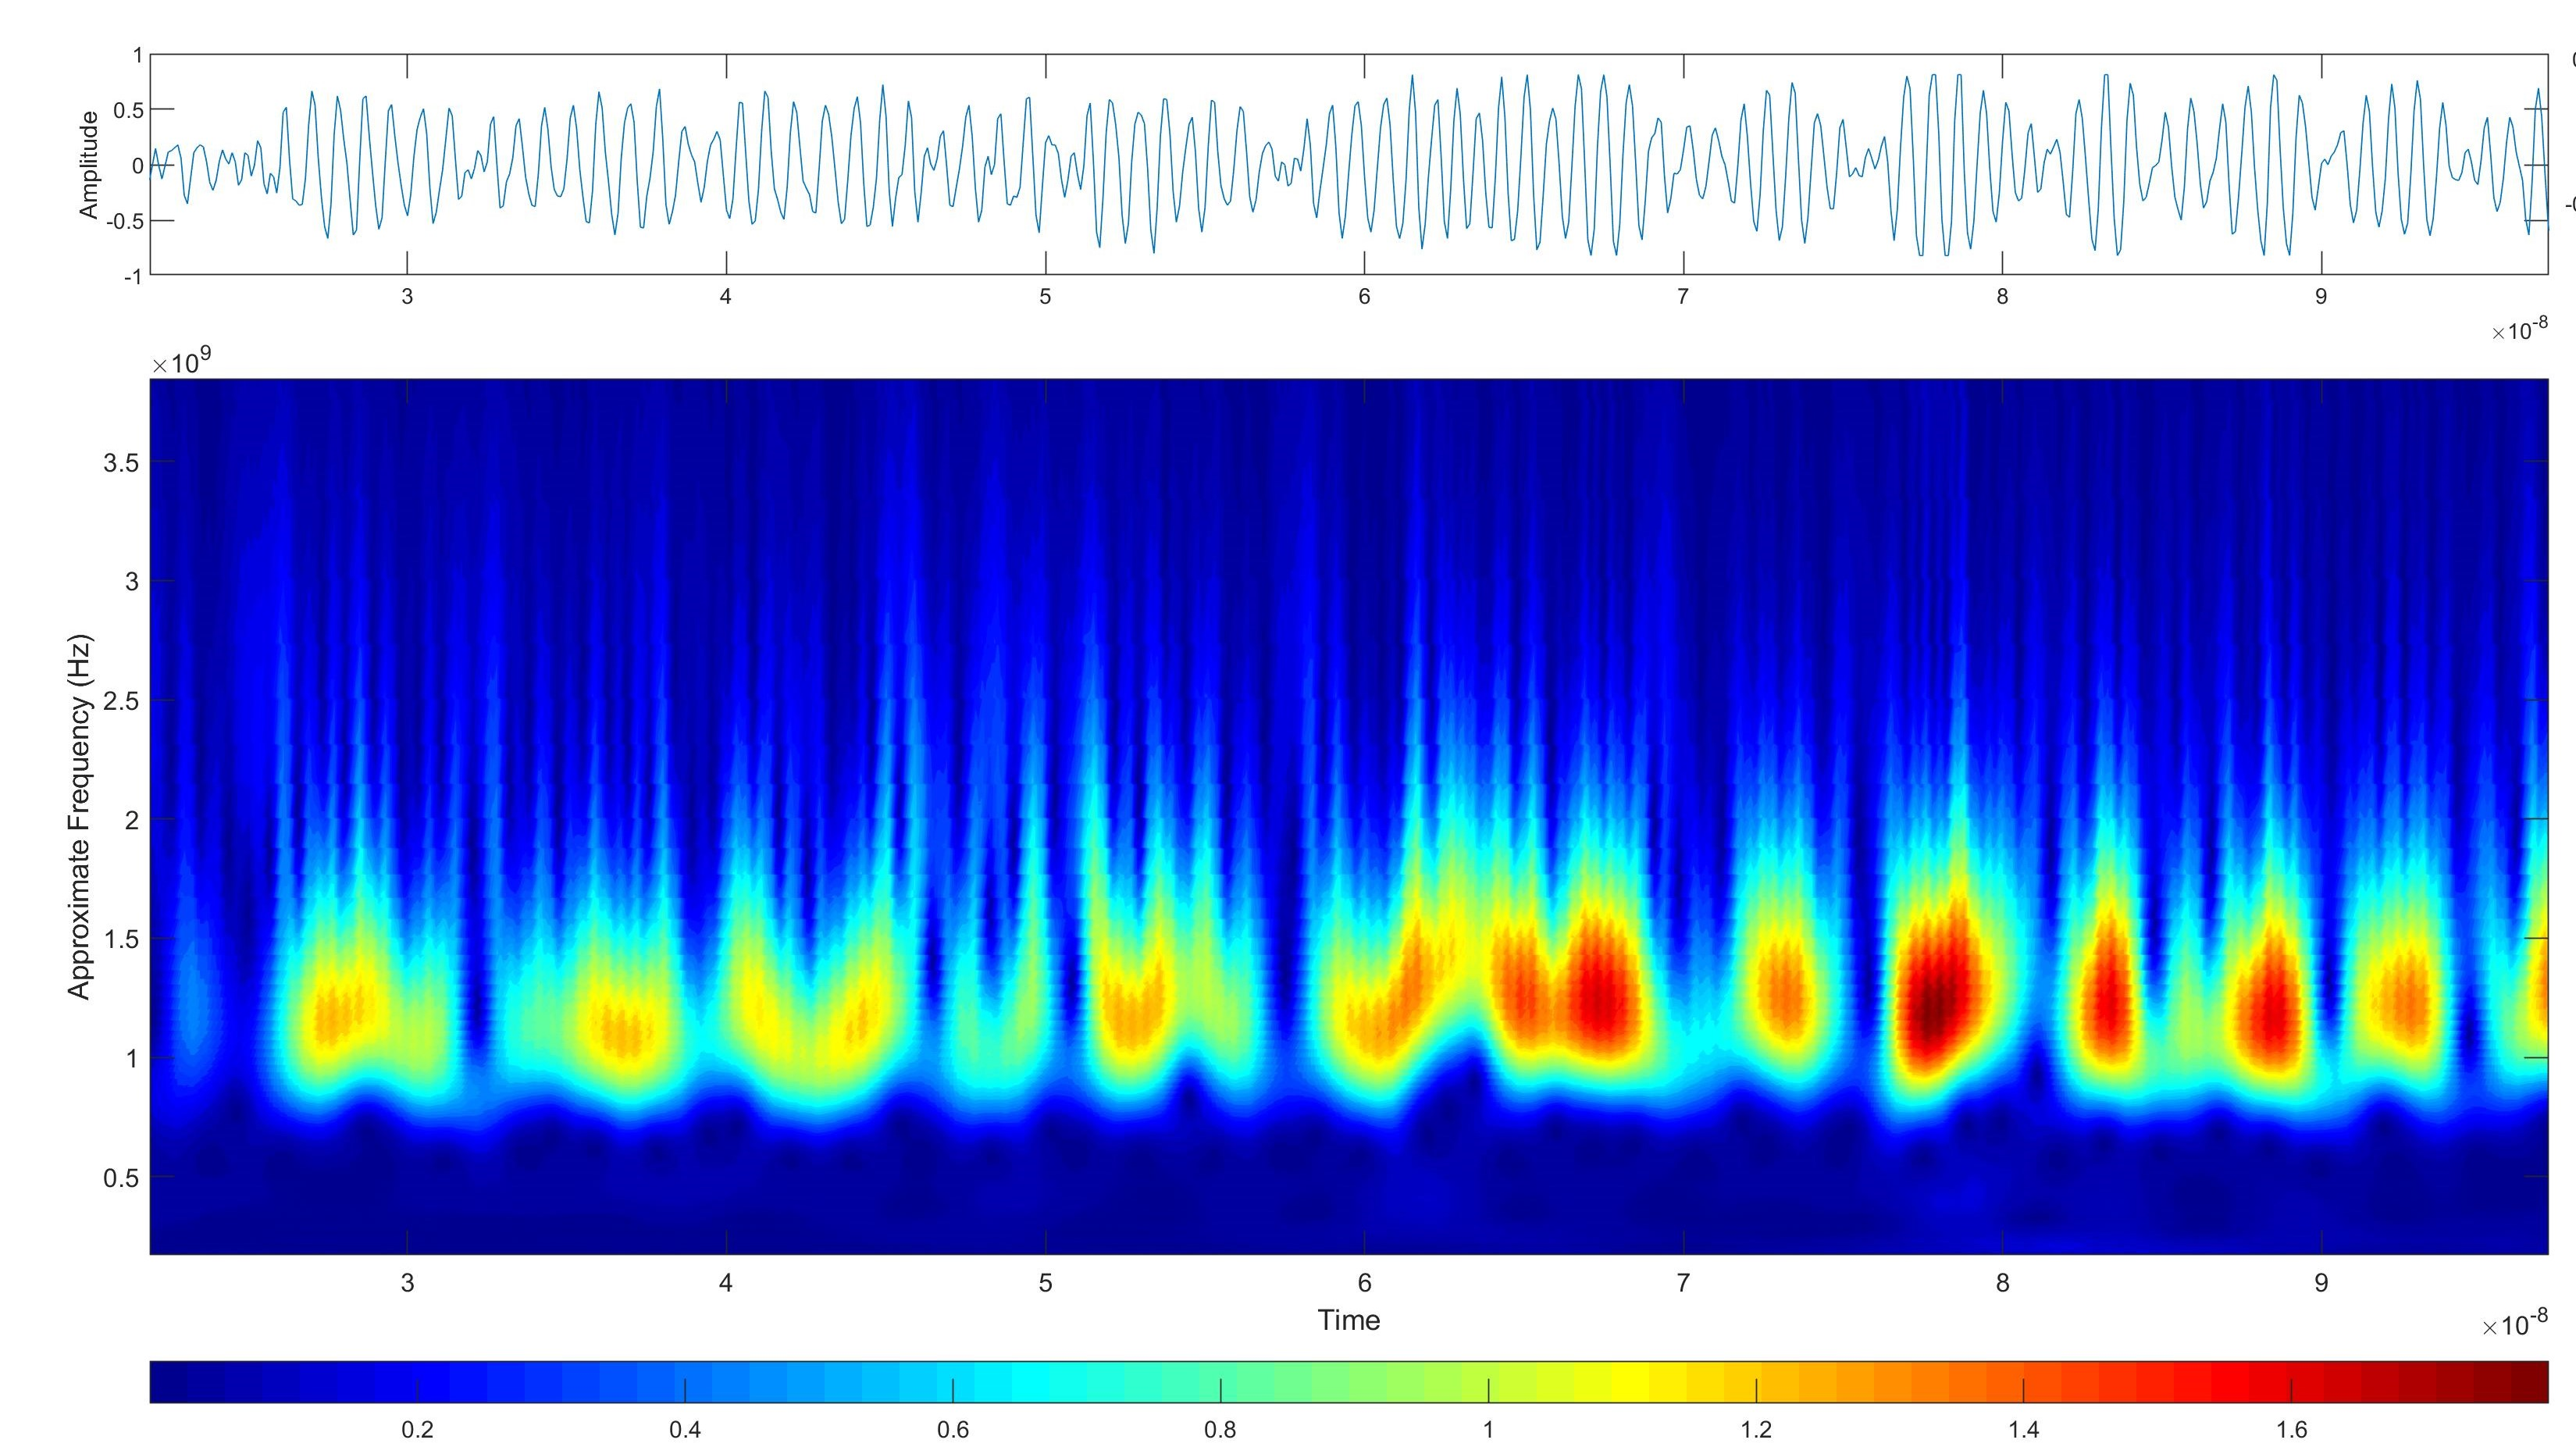
\includegraphics[width=1\linewidth]{papers/gis/Bilder/cgau5}
	\captionof{figure}{CWT Plot komplexes Gausches-Wavelet Nr.5}
	\label{fig:cgau5}
\end{figure}

Mit einem Haar-Wavelet erhält man eine sehr hohe Zeitauflösung zu welchem Zeitpunkt ein Event stattgefunden hat.
Mit einem Morlet-Wavelet wird die Frequenzauflösung erhöht, jedoch resultiert eine ungenauere Zeitauflösung.
Mit zwei Graphen, ist die Unschärferelation in den Abbildungen \ref{fig:UnschRelMorl} und \ref{fig:UnschRelHaar} veranschaulicht. 
Der CWT Plot vom Haar-Wavelet weist scharfe Kanten auf, welche gut mit den Minimas und Maximas des Zeitsignals korrelieren.
Die Frequenzen sind jedoch über den Frequenzbereich verschmiert, diese Auflösung ist beim Morlet-Wavelet höher.

Bei den reellwertigen Wavelets ist immer auch eine 'Perlenketten' ähnliche Struktur erkennbar (siehe Plots in Abbildungen \ref{fig:UnschRelHaar} und \ref{fig:UnschRelMorl}).
Ohne tiefere Überlegung könnte man versucht sein diese Struktur als mögliches fehlertypisches Merkmal zu interpretieren. 
Bei genauerer Betrachtung wird jedoch klar, dass sich die Perlenketten zwischen den Nullstellen vom Zeitsignal befinden und sie keine brauchbare Information für das beschriebene Problem beinhalten.
Die Perlenkettenbildung zwischen den Nullstellen kann umgangen werden wenn die CWT mit einem komplexen Wavelet durchgeführt wird.
Interessant dabei ist, dass nun Schwebungen im Zeitsignal zu einer quasi abgeschlossenen Kontur im CWT Plot führen.
Dies ist gut erkennbar in der Abbildung \ref{fig:cgau5} im Zeitintervall von 28ns bis 33ns.

\section{Schlussfolgerung}
\rhead{Schlussfolgerung}
Das Ziel dieser Arbeit war aus Zeitsignalen fehlerspezifische Charakteristiken zu extrahieren mit Hilfe der CWT Analyse.
Die verwendeten Signale stammen von TOF-Aufzeichnungen, welche während der TE-Analyse bei einer Anlage im Betrieb aufgezeichnet wurden. Es bestand Klarheit über die Teilentladungsquelle und die damit verbundene Fehlerart. 
Es wurde auf die physikalischen wie elektrotechnischen fehlerspezifische Phänomene eingegangen, mit dem Ziel aus diesen Erkenntnissen Rückschlüsse auf die CWT Plots ziehn zu können.

In der Analyse des Messpfades wurde der Ausbreitungsweg elektromagnetischer Wellen innerhalb und ausserhalb einer GIS aufgezeigt.
Hier wurde klar, dass das Finden von fehlerspezifische Charakteristiken im CWT Plot schwierig sein wird.
Dies aufgrund der Tatsache, dass die GIS nicht als Koaxialkabel mit konstantem Wellenwiderstand betrachtet werden kann und sich die Fehlstelle nicht in naher Umgebung der Koppelantenne befinden.
Die Signale werden von der Fehlerquelle bis zur Koppelantenne aufgrund von Refelxions- und Dispersionsphänomenen (frequenzabhängige Laufzeiten) stark verzerrt und die ursprüngliche Form geht verloren.
Die Verzerrung des Signals ist ersichtlich, wenn die Bilder vom Signalpuls an der Fehlstelle \ref{fig:Teilentaldungspuls} und dem Signal der Koppelantenne \ref{fig:Zeitsig} verglichen wird.

Bei der optischen Analyse beider Fehlerarten wurden keine Auffälligkeiten in den CWT Plots entdeckt. 
Der Autor geht davon aus, dass dieses Resultat auf die erwähnte Signalverzerrung zurückzuschliessen ist und der Signalpfad innerhalb der GIS zu viele Unstetigkeitsstellen aufweist.

Bei der Beurteilung der Resultate welche in dieser Arbeit vorliegen, sollte jedoch in Betracht gezogen werden, dass vielleicht mit einer breiteren Datenbasis und Machine Learning fehlerspezifische Charakteristiken herausgefiltert werden könnten. 

\section{Danksagung}
Ein grosser Dank geht an Glenn Behrmann von der Firma ABB Schweiz AG. 
Er hat die Aufzeichnungen zur Verfügung gestellt und wir hatten beim Projektstart interessante Diskussionen. An dieser Stelle möchte ich erwähnen, dass Herr Behrmann mich von Beginn an auf das Problem der Signalverzerrung aufmerksam gemacht hat.

\begin{figure}
	\centering
    \begin{tikzpicture}
	\begin{axis}
	[
	width = 10cm,
	height = 4cm,
	xmin =0,
	xmax = 1.6,
	xlabel= Zeit (ns),
	ylabel= TE Strom (mA)
	]
	\addplot [black, samples=10000] file {papers/gis/Messdaten/PDpuls.txt};
	\end{axis}
	\end{tikzpicture}
    \caption{Teilentladungspuls an der Fehlstelle (Koronaentladung) \cite{skript:Judd24ps}}
	\label{fig:Teilentaldungspuls}
\end{figure}

\printbibliography[heading=subbibliography]
\end{refsection}
